{\descr{Провести повне дослідження функції і побудувати графік}}

$$
y=\dfrac{2}{x^2+2x}
$$


1) $x \in (-\infty;-2)\cup(-2;0)\cup(0;+\infty)$

2) Графік не перетинає ось $x$.

3) Функція непарна оскільки

$$
  f(-x) = \dfrac{2}{(-x)^2+2(-x)} = \dfrac{2}{x^2-2x}
$$

4) Обидві точки -2 та 0 носить характер розриву другого роду оскільки вони прямують в безмежність.

$$
  \lim_{x \to -2 \ \pm0} \dfrac{2}{x^2+2x} = \mp \infty \qquad   \lim_{x \to 0 \ \pm0} \dfrac{2}{x^2+2x} = \pm \infty
$$

5) Похідна
$$
  y' = (\dfrac{2}{x^2+2x})'
     = \dfrac{2'(x^2+2x)-2(x^2+2x)'}{(x^2+2x)^2}
     = \dfrac{-4x-4}{(x^2+2x)^2}
$$

Функція не існує в точках $x=-2$ та $x=0$, а $x=-1$ є критичною (такою що є підозрілою на екстремум мінімум або максимум). На інтервалі $(-\infty;+\infty)$ матимемо:



\begin{center}
  \begin{tabular}{ | c | c | c | c | c | c | c | c | }
    \hline
      x     & (-\infty;-2) & -2 & (-2;-1) & -1 & (-1:0) & 0 &  (0; +\infty) \\
      \hline
      f'(x) &  + & не існує & + & 0  & -  & не існує & - \\
      \hline
      f(x)  & \nearrow  & не існує & \nearrow  & y_{max} = -2  & \searrow   & не існує & \searrow \\
    \hline
  \end{tabular}
\end{center}



6) Друга похідна

$$
  y'' = (\dfrac{-4x-4}{(x^2+2x)^2})'
  = \dfrac{(-4x-4)'(x^2+2x)^2 - (-4x-4)((x^2+2x)^2)' }{(x^2+2x)^4}
$$

$$
= \dfrac{-4(x^2+2x) + 4(2x+2)^2 }{(x^2+2x)^3}
= \dfrac{-4x^2-8x + 16x^2+32x+16 }{(x^2+2x)^3}
= \dfrac{12x^2+24x+16 }{(x^2+2x)^3}
$$

\begin{center}
  \begin{tabular}{ | c | c | c | c | c | c |  }
    \hline
    x & (-\infty;-2) & -2 & (-2:0) & 0 & (0:+\infty) \\
    \hline
    f"(x) &  + & не існує  & - & не існує & +  \\
    \hline
    f(x) &  \cup & не існує  & \cap & не існує & \cup \\
    \hline
  \end{tabular}
\end{center}

7) з пункта (4) випливає що фунція має вертикальні асимптоти в точках $x=-2$ та $x=0$.

Знаходимо горизонтальні асимптоти за формулами (через границі функції):
$$
  y = kx+b
$$

$$
  k = \lim_{x\to\infty} \dfrac{y(x)}{x}
    = \lim_{x\to\infty} \dfrac{2}{x(x^2+2x)}
    = \lim_{x\to\infty} \dfrac{2/x^2}{x(1+2/x)}
    = \dfrac{1}{\infty}
    = 0
$$

$$
  b = \lim_{x\to\infty} (y(x) - kx)
    = \lim_{x\to\infty} \dfrac{2}{x^2+2x}
    = \lim_{x\to\infty} \dfrac{2/x^2}{1+2/x}
    = \dfrac{0}{1}
    = 0
$$

8) Враховуючи висновки ослідження функції будуємо графік:

\begin{figure}[h!]
  \centering
  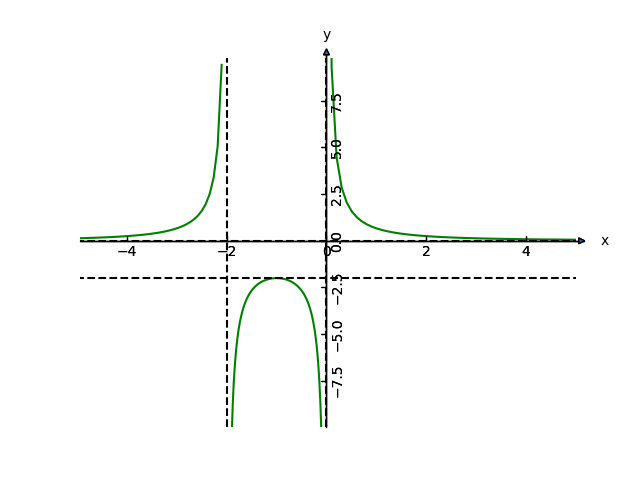
\includegraphics[width=14cm]{rozrahunkova_01/07_01.png}
  \caption{Графік функції $y=\dfrac{2}{x^2+2x}$ }
  \label{fig:rr_01_07_01}
  \centering
\end{figure}
